\documentclass[a4paper, 11pt]{article}
\usepackage[utf8]{inputenc}
\usepackage{amsmath}
\usepackage{array}
\usepackage{listings}
\usepackage{color}
\usepackage{booktabs}
\usepackage{caption}
\usepackage{varioref}
\usepackage[section]{placeins}
\usepackage{comment} % enables the use of multi-line comments (\ifx \fi) 
\usepackage{graphicx}
\usepackage{lipsum} %This package just generates Lorem Ipsum filler text. 
\usepackage{fullpage} % changes the margin
\usepackage{cleveref}
\definecolor{dkgreen}{rgb}{0,0.6,0}
\definecolor{gray}{rgb}{0.5,0.5,0.5}
\definecolor{mauve}{rgb}{0.58,0,0.82}

\DeclareMathOperator*{\argmax}{argmax} % thin space, limits underneath in displays

\newenvironment{conditions}
{\par\vspace{\abovedisplayskip}\noindent\begin{tabular}{>{$}l<{$} @{${}={}$} l}}
	{\end{tabular}\par\vspace{\belowdisplayskip}}

\renewcommand{\lstlistingname}{Algorithm}% Listing -> Algorithm
\renewcommand{\lstlistlistingname}{List of \lstlistingname s}% List of Listings -> List of Algorithms
\crefname{listing}{algorithm}{algorithms}  
\Crefname{listing}{Algorithm}{Algorithms}

\lstset{frame=tb,
	language=Python,
	aboveskip=3mm,
	belowskip=3mm,
	showstringspaces=false,
	columns=flexible,
	basicstyle={\small\ttfamily},
	numbers=left,
	numberstyle=\tiny\color{gray},
	keywordstyle=\color{blue},
	commentstyle=\color{dkgreen},
	stringstyle=\color{mauve},
	breaklines=true,
	breakatwhitespace=true,
	tabsize=3,
	inputencoding=latin1
}

\captionsetup[figure]{skip=0pt}

\begin{document}
	%Header-Make sure you update this information!!!!
	\noindent
	\large\textbf{Homework 2 Report} \hfill \textbf{Piero Macaluso s252894} \\
	\normalsize Machine Learning and Artificial Intelligence 2018/2019 \hfill Due Date: 19/01/2019 \\
	Prof. Barbara Caputo  
	
	\section{Linear SVM} \label{linearsvm}
	
	In the first part of this homework I trained, validated and finally tested a Linear SVM, using the $C$ with the highest accuracy in validation. The essential part of the code is \vref{lst:linear}.
	
	\lstinputlisting[linerange={78-104},firstnumber=78,label={lst:linear},caption={Searching the best value of C in Linear SVM}]{../source_code/main.py}
%	\lstinputlisting[linerange={87-110},firstnumber=87,label={lst:linear},caption={Searching the best value of C},belowskip={1pt}]{../source_code/main.py}
%	\lstinputlisting[linerange={109-110},firstnumber=109=label={lst:linear},aboveskip={1pt}]{../source_code/main.py}
	
	As we can see from the plots \vref{fig:linear1,fig:linear2}, the best accuracy found on validation set was $\boldsymbol{73.33\%}$, with $C$ equal to  $\boldsymbol{1\mathrm{e}{-1}}$. I noticed that boundaries became more and more precise on the training set with the increment of $C$. 
	
	$C$ is the hyper parameter of SVM that represents the penalty for misclassifying a data point, so it describe how much we want to avoid misclassification during the training.
	\textbf{When $\boldsymbol{C}$ is large}, the optimization will choose a smaller-margin hyperplane, because the classifier is heavily penalized for misclassified data.
	The larger is $C$, the better the classification on training set will be. On the contrary, when \textbf{$\boldsymbol{C}$ is small}, the optimizer will use a larger-margin separating hyperplane, causing the misclassification of more training data points.
	
	After this training, I tests the data on the test set obtaining a greater accuracy, it goes very well with an accuracy of $\boldsymbol{88.89\%}$ as we can see in \vref{fig:linear3}.  I tried to repeat the code a lot of times using a different \texttt{random\_state} variable, obtaining validation values from $60\%$ to $90\%$. This may be due to the initial state of the algorithm of SVM or the splitting of the data in training, validation and test sets: maybe one time the is more overfitting on the training data, next time less. We may conclude that this type of validation is not stable and may be influenced by overfitting (see \vref{final}).

	
	\begin{figure}[ht!]
		\centering
		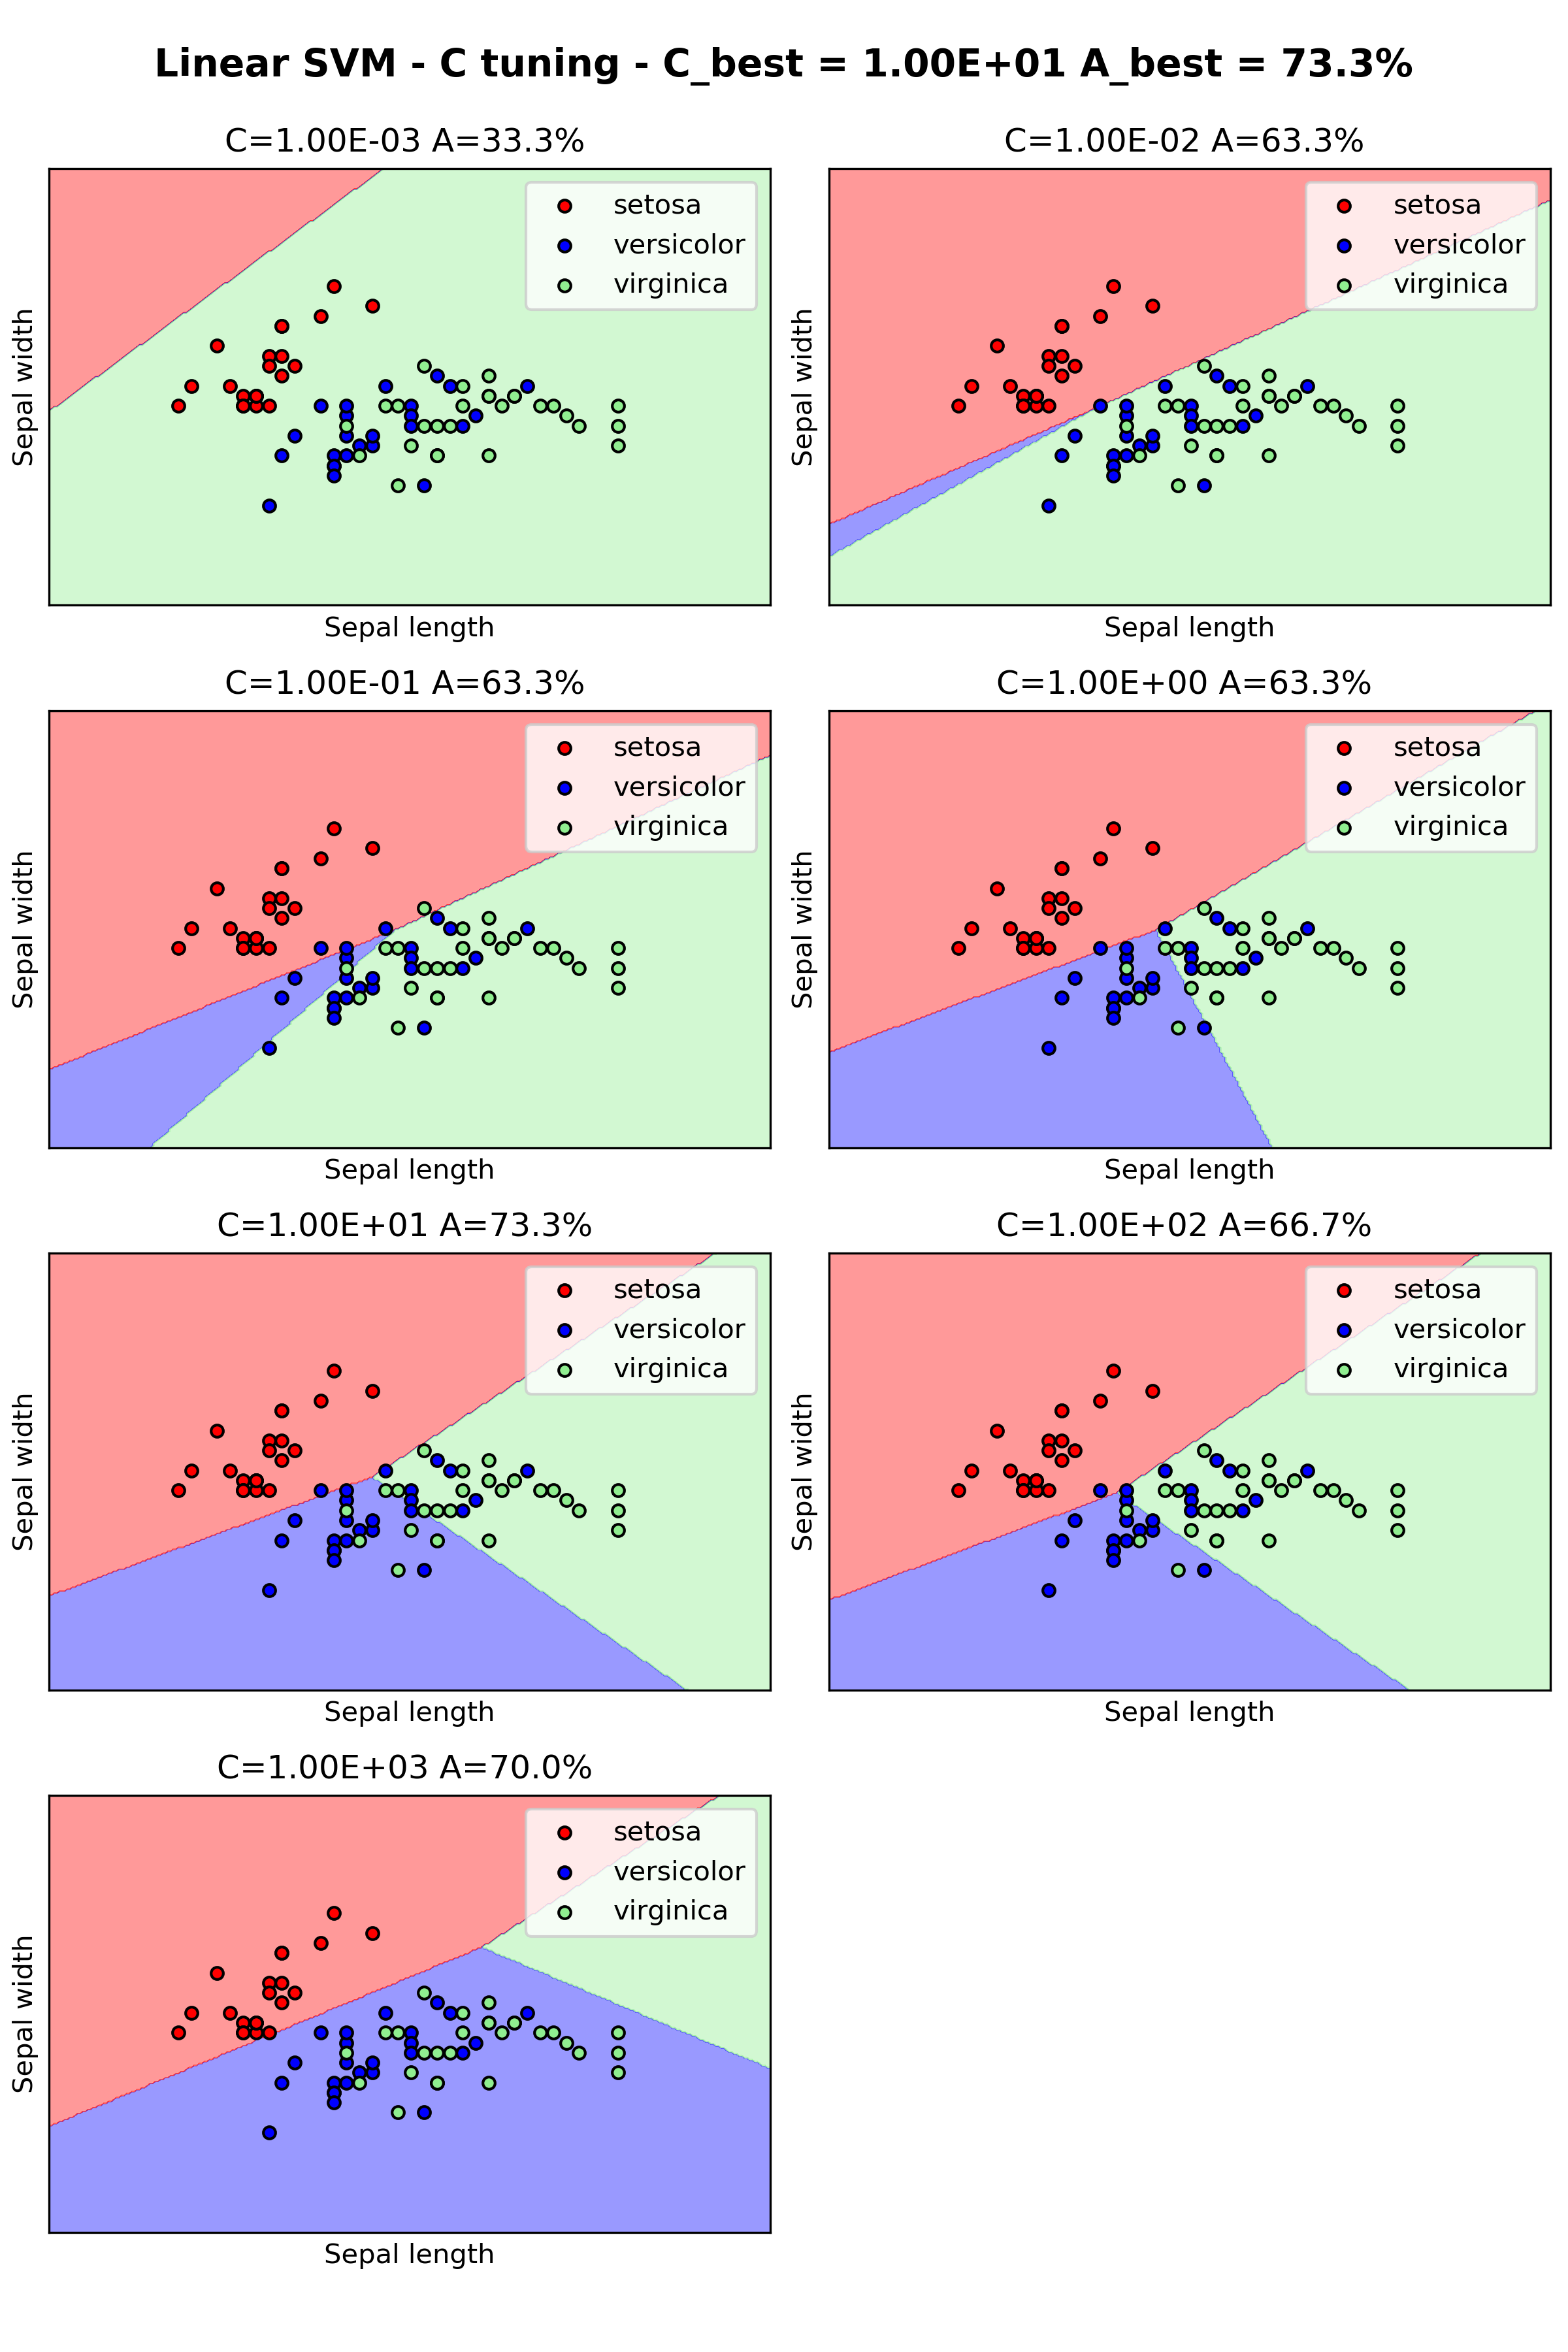
\includegraphics[height=0.8\paperheight]{img/fig01a.png}
		\caption{Decision Boundaries changing C in Linear SVM on Training set}
		\label{fig:linear1}
	\end{figure}

	\begin{figure}[ht!]
		\centering
		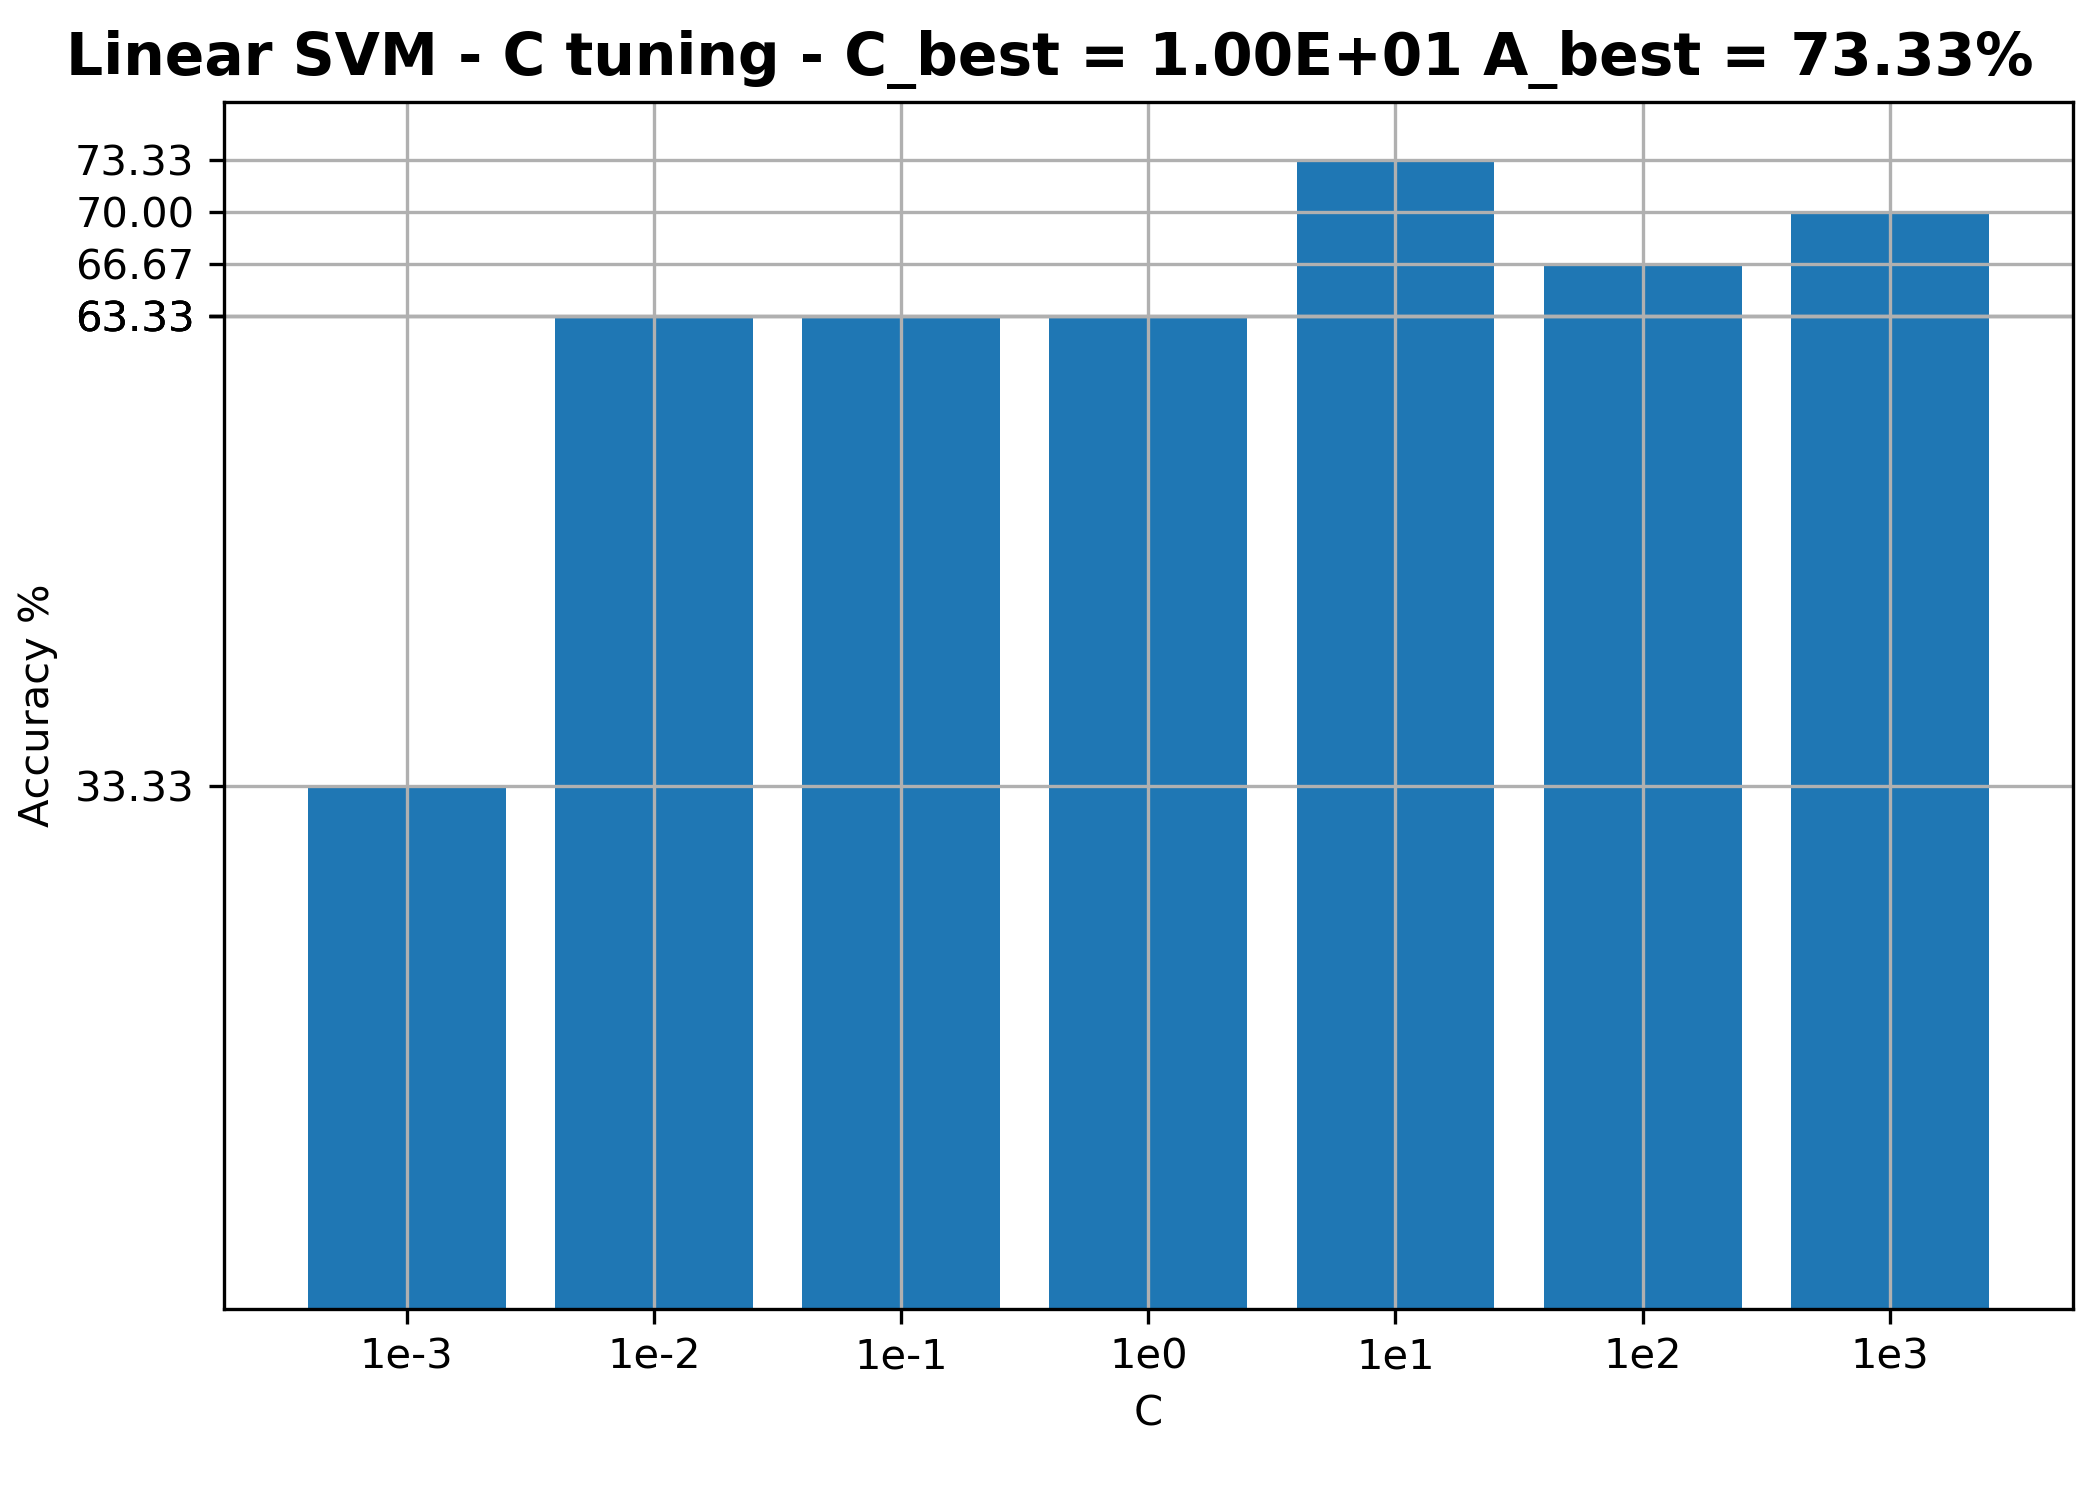
\includegraphics[width=0.7\paperwidth]{img/fig01b.png}
		\caption{Accuracy changing C in Linear SVM}
		\label{fig:linear2}
	\end{figure}

	\begin{figure}[ht!]
		\centering
		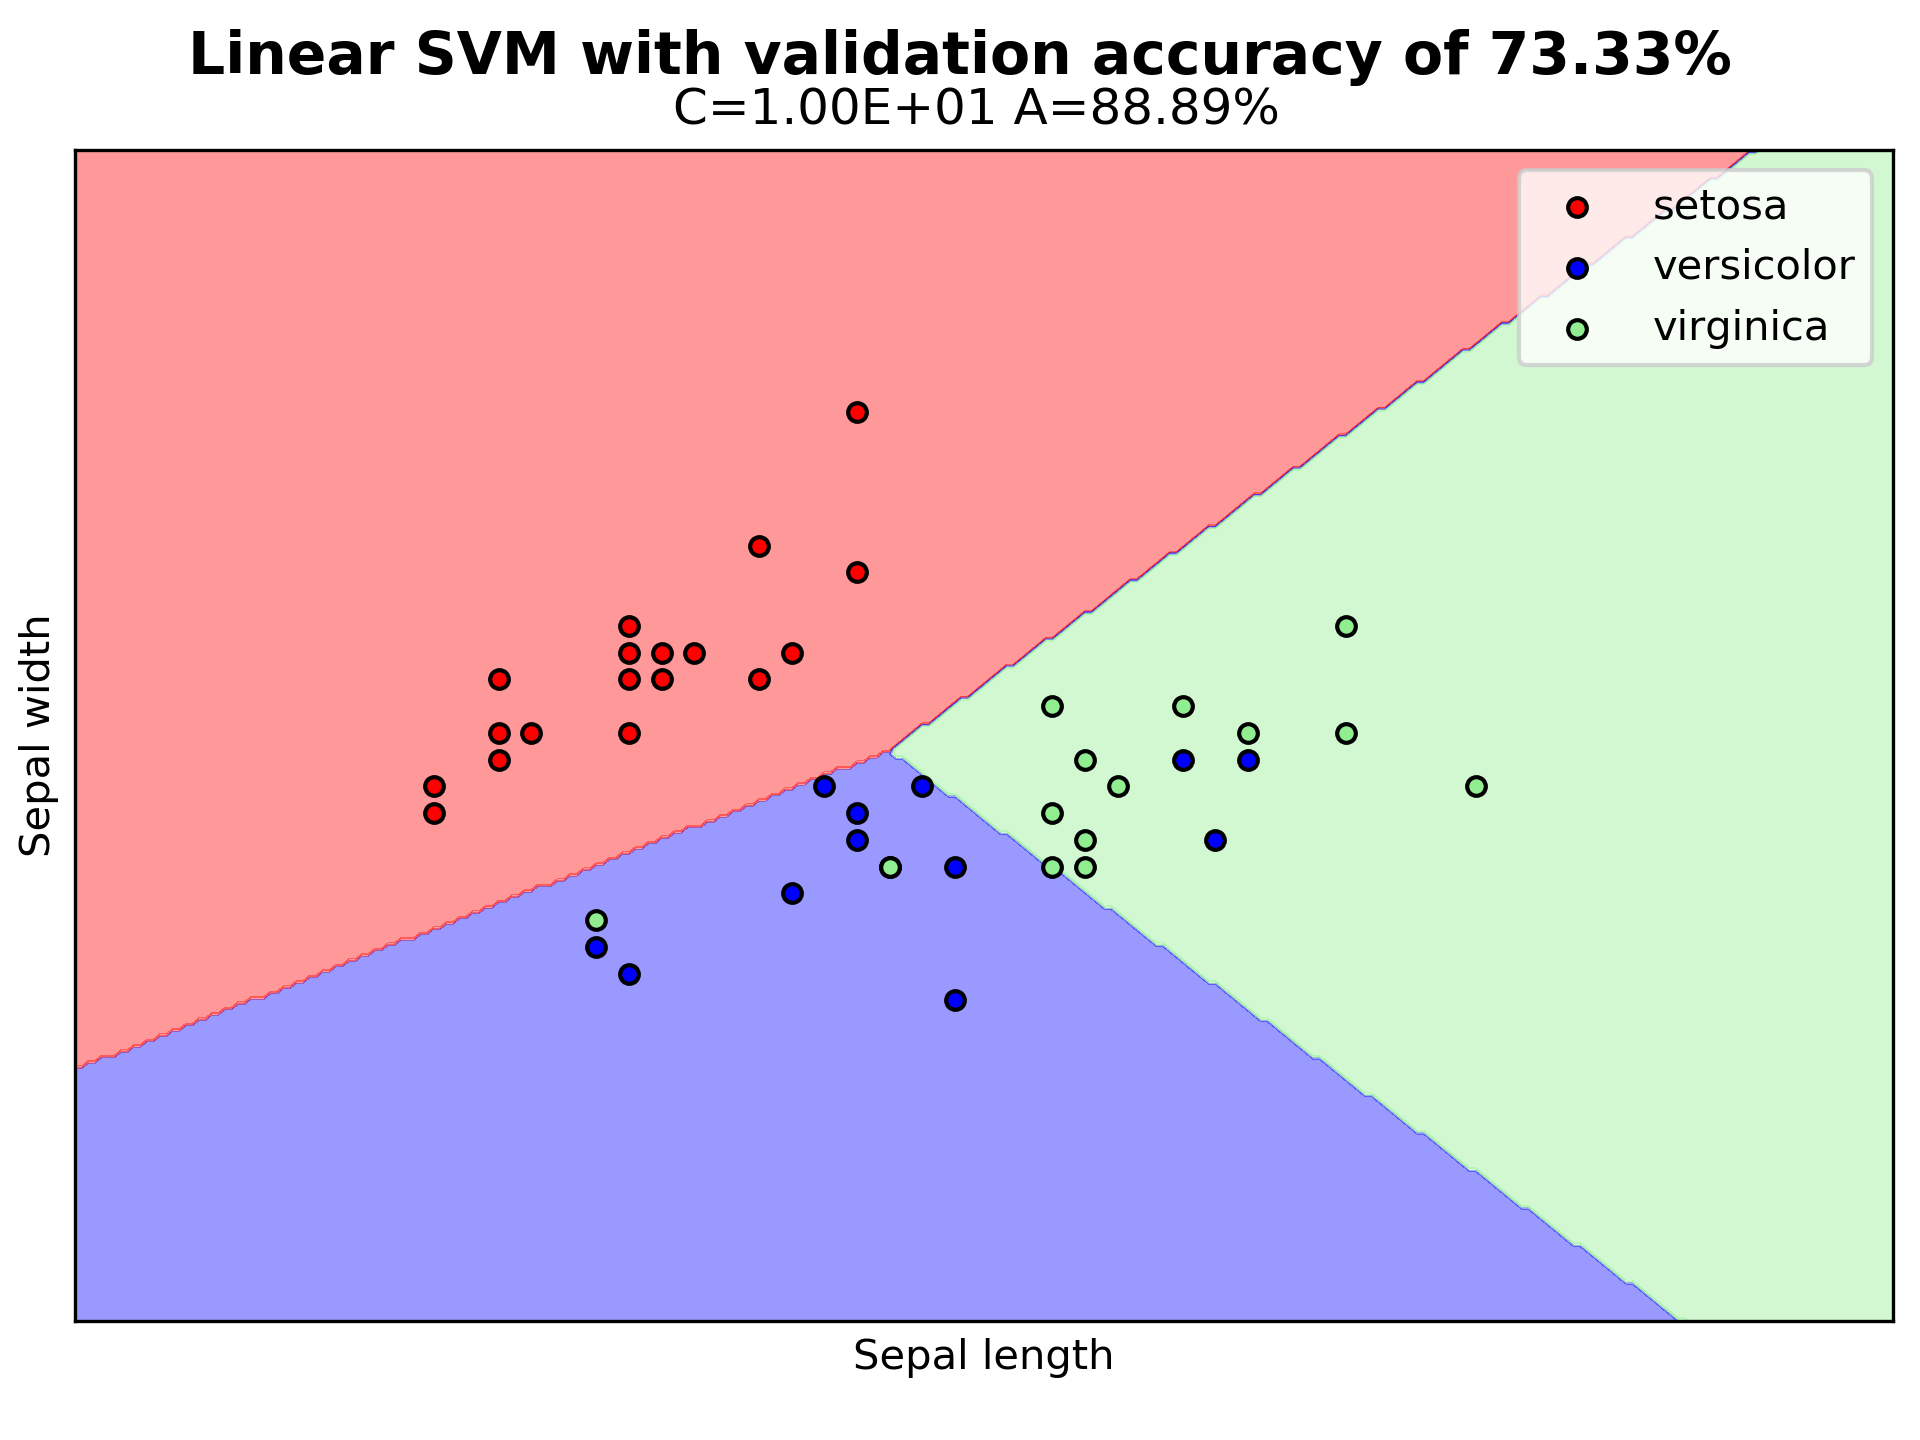
\includegraphics[width=0.7\paperwidth]{img/fig01c.png}
		\caption{Results on the test set}
		\label{fig:linear3}
	\end{figure}
		
	\section{RBF Kernel}
	
	In the second part of this homework, I used SVM with \textbf{Gaussian RBF kernel} \vref{eq:1}.
	\begin{equation} \label{eq:1}
	exp(-\gamma \mid\mid x-x' \mid\mid^2)
	\end{equation}
	This time I had to find the best pair of $C$ (explained in \vref{linearsvm})  and $\gamma$ (Gamma).
	
	\textbf{Gamma parameter} can be explained as the \textit{spread} of the kernel and therefore the decision region. When gamma is \textbf{low}, the \textit{curve} of the decision boundary is very low and thus the decision region is very broad. When gamma is \textbf{high}, the \textit{curve} of the decision boundary is high, which creates islands of decision-boundaries around data points.
	
	Firstly, I repeated the steps of the previous section in order to find the best accuracy modifying $C$ and using the Gamma calculated by \texttt{sklearn} under the hood as we can see in \vref{lst:rbf1}.  This time the boundaries are \textbf{not as linear as} the ones of Linear SVM because of the introduction of the Gaussian RBF kernel. Thanks to this approach, I found a better training accuracy ($\boldsymbol{76.67\%}$) compared to the Linear SVM one, and a test accuracy near to the validation one ($\boldsymbol{75.56\%}$) with $\boldsymbol{C=1\mathrm{e}{-1}}$ as we can see in \vref{fig:rbf1,fig:rbf2,fig:rbf3}.
	
	I used the the code of \vref{lst:linear} changing the classifier on line $88$ with the one in \vref{lst:rbf1} .
	
	\lstinputlisting[linerange={152-152},firstnumber=152,label={lst:rbf1},caption={RBF Kernel SVM Classifier}]{../source_code/main.py}
	
	Finally, I performed the grid search of the best pair of $C$ and $Gamma$ with \vref{lst:rbf2}. This time I obtained an high accuracy in validation ($\boldsymbol{80.00\%}$) and also on the test set ($\boldsymbol{86.67\%}$) with a $\boldsymbol{C=1\mathrm{e}{0}}$ and $\boldsymbol{\gamma=1\mathrm{e}{-1}}$ as we can see in \vref{fig:rbf4,fig:rbf5}.
	
	\lstinputlisting[ linerange={211-227},firstnumber=211,label={lst:rbf2},caption={Searching the best value of C and Gamma in RBF Kernel SVM}]{../source_code/main.py}
	
	I repeated this code a lot of times and, even then, I found a great variation of results in validation and test scores (see \vref{final}).
	
	\begin{figure}[ht!]
		\centering
		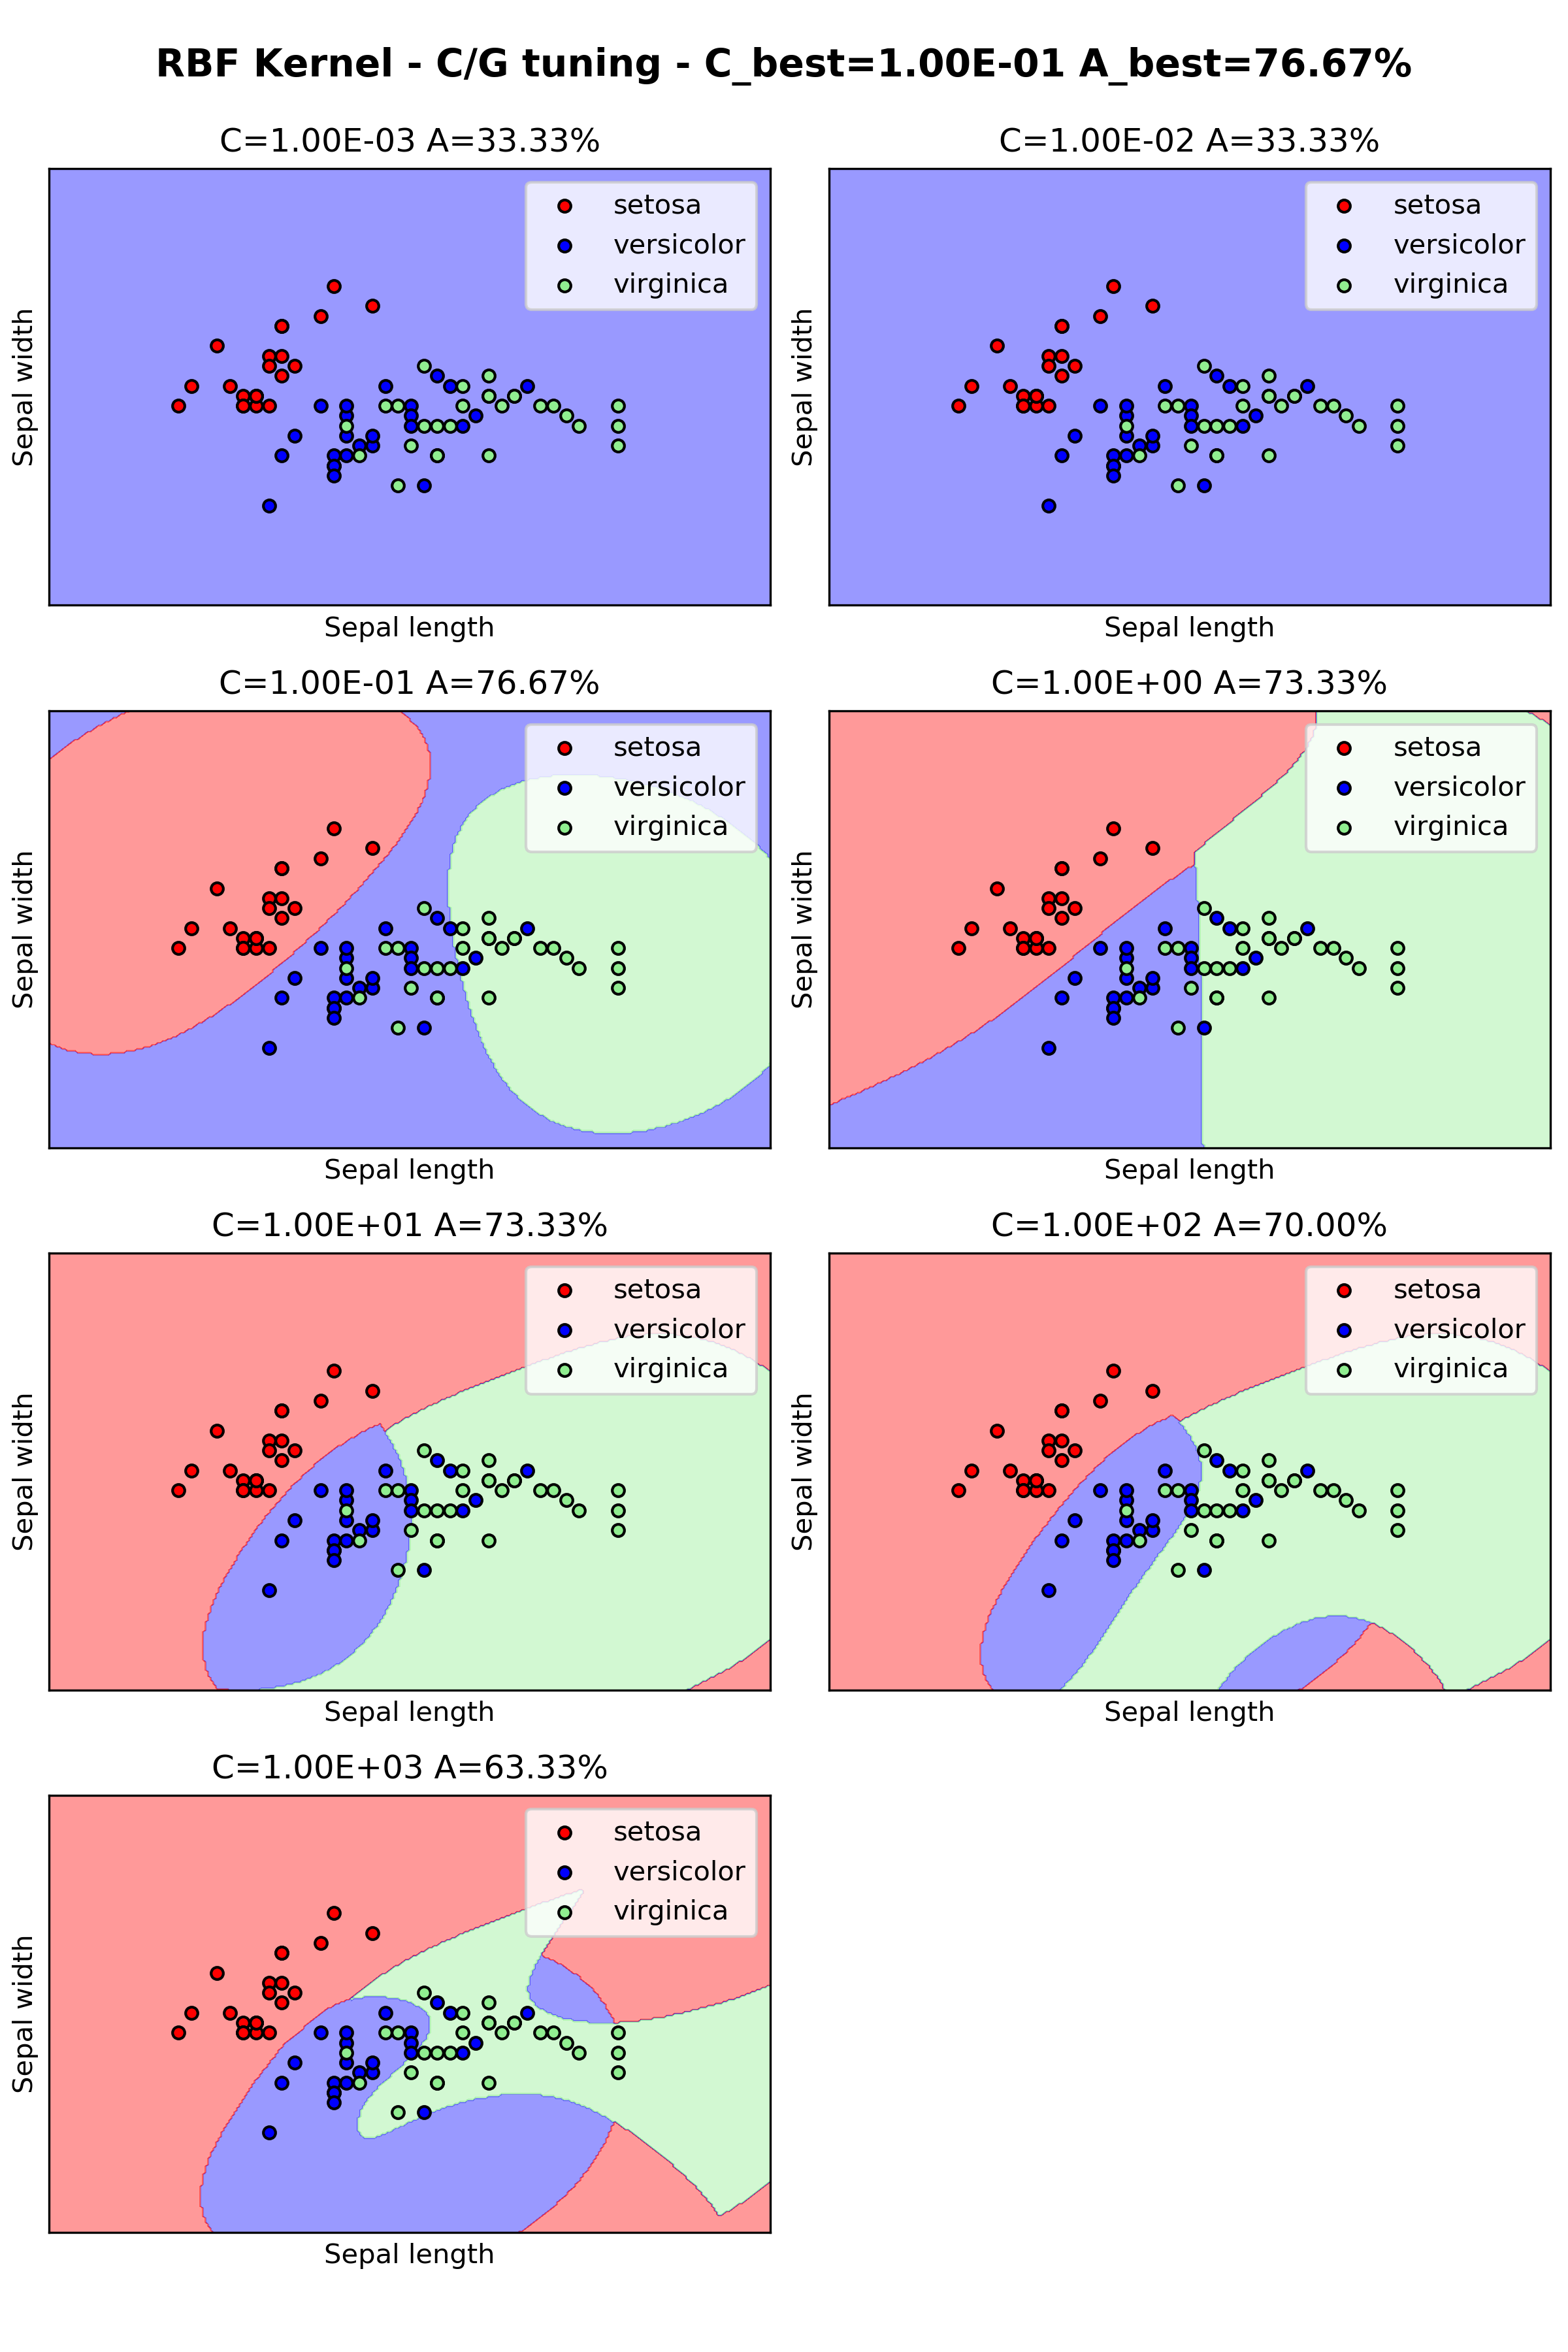
\includegraphics[height=0.8\paperheight]{img/fig02a.png}
		\caption{Decision Boundaries changing C in RBF Kernel SVM on Training set}
		\label{fig:rbf1}
	\end{figure}
	
	\begin{figure}[ht!]
		\centering
		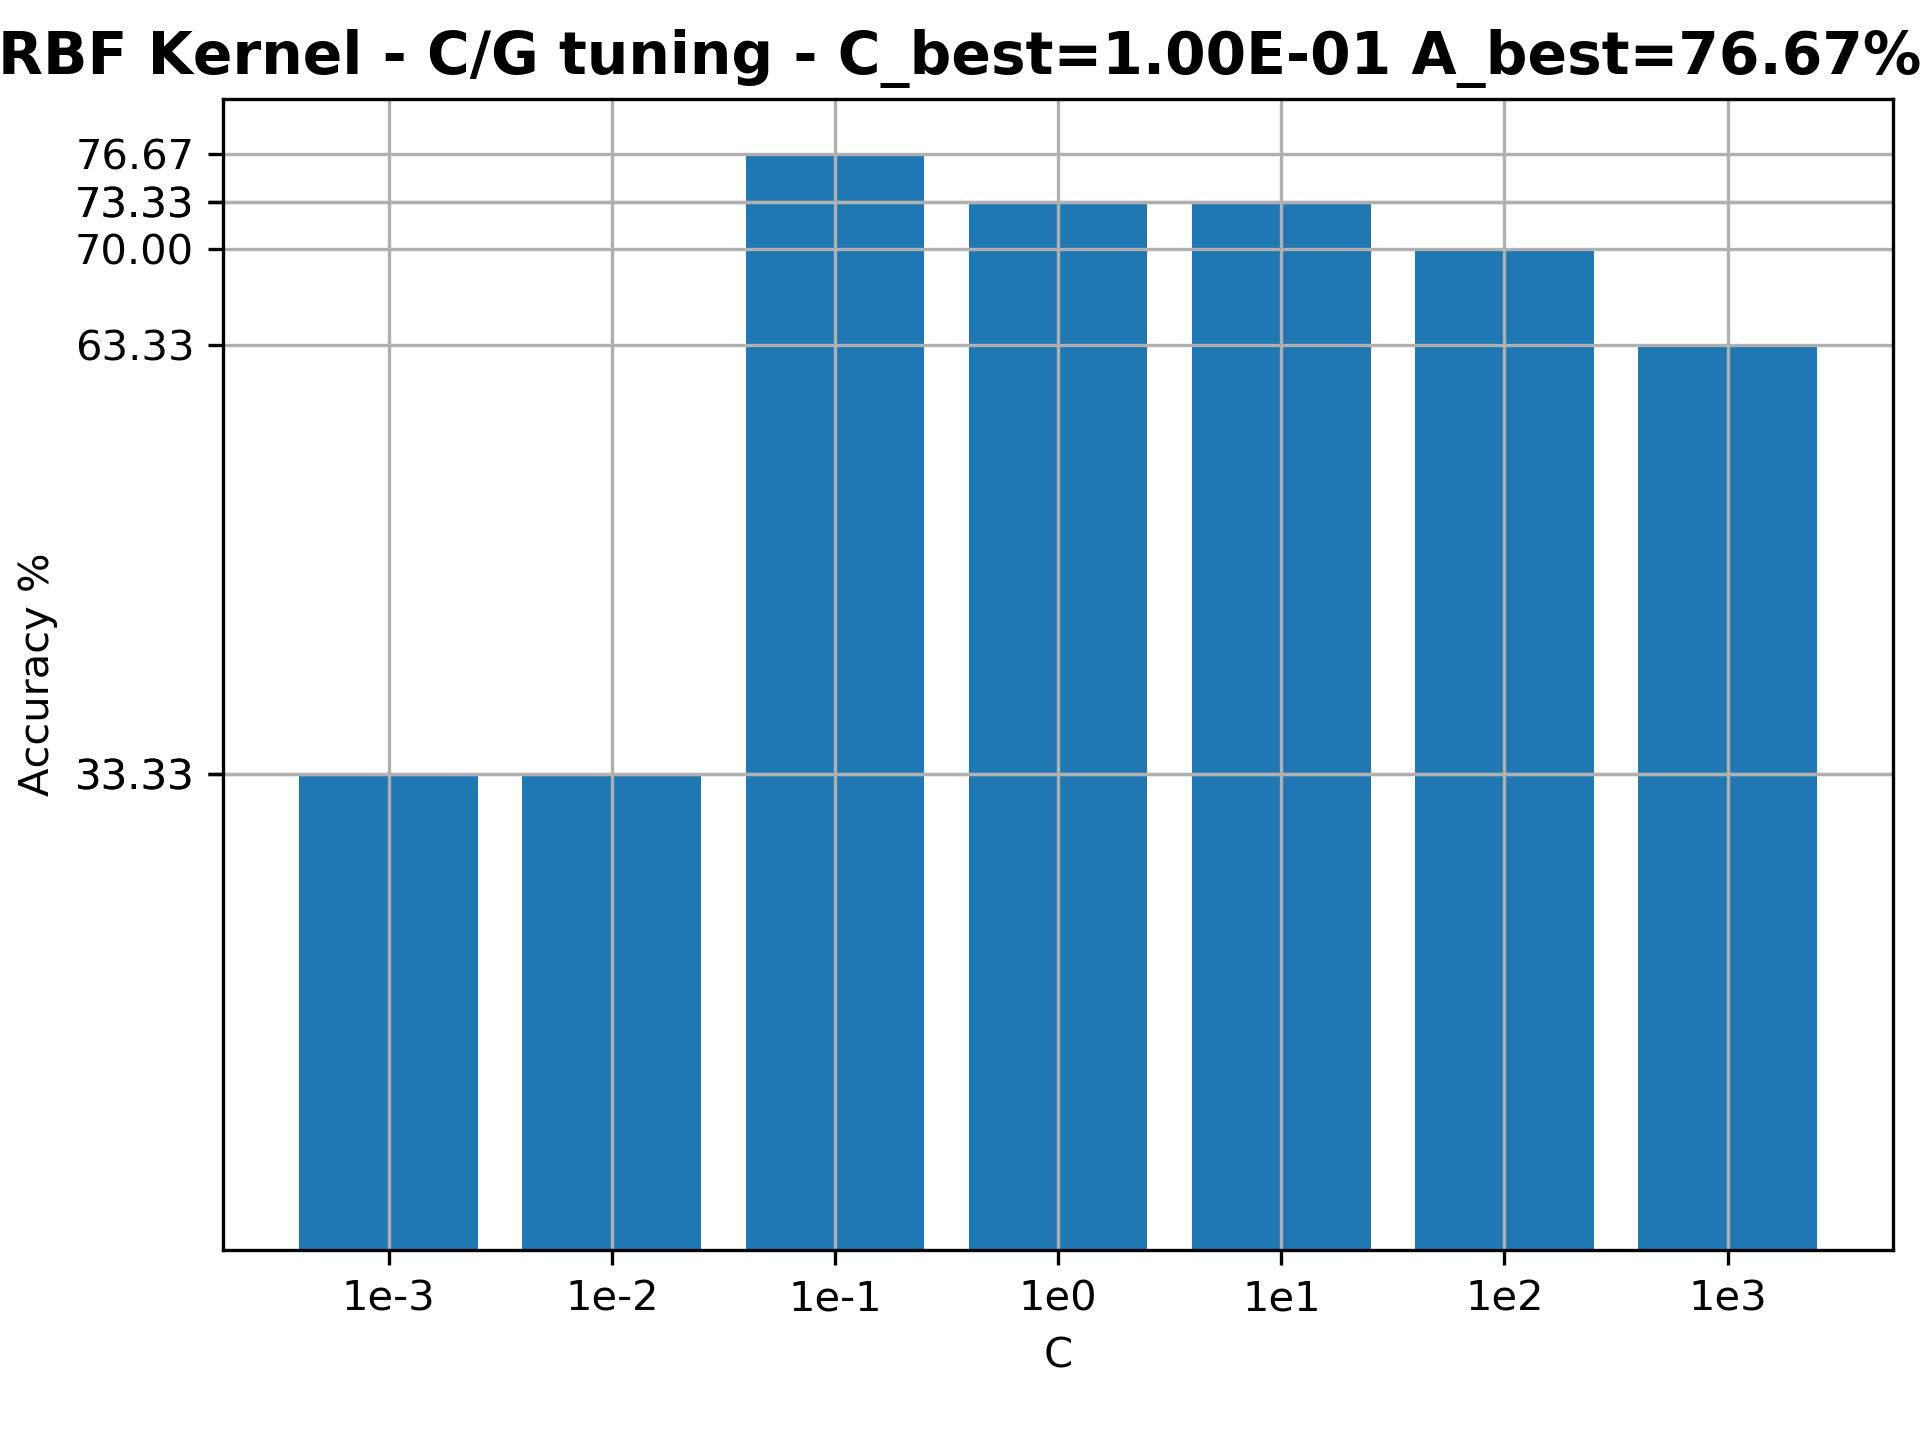
\includegraphics[width=0.7\paperwidth]{img/fig02b.png}
		\caption{Accuracy changing C in RBF Kernel SVM }
		\label{fig:rbf2}
	\end{figure}
	\begin{figure}[ht!]
		\centering
		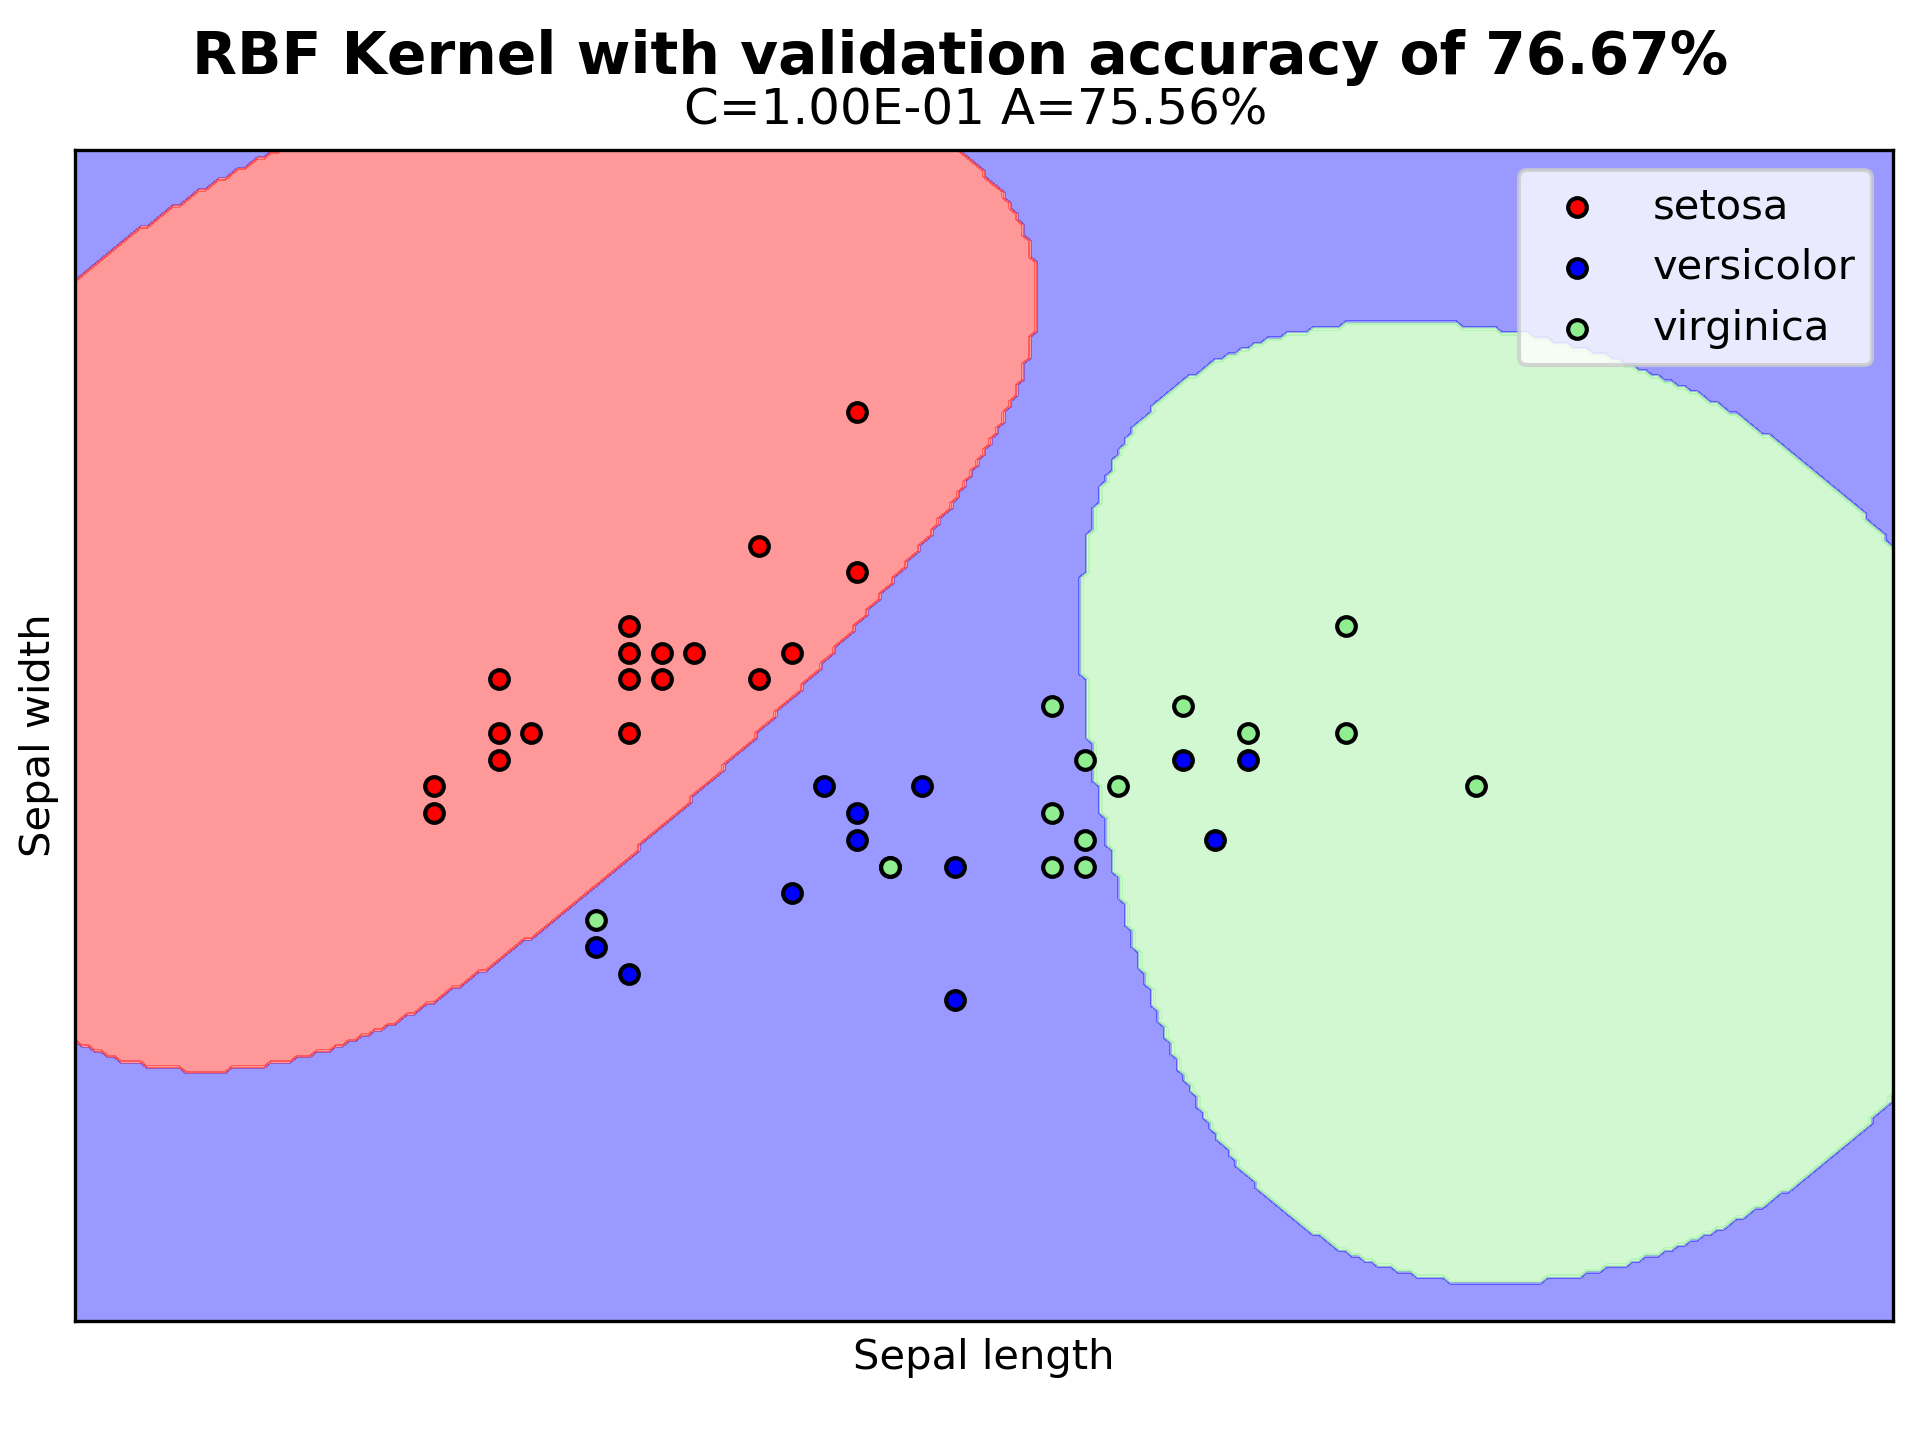
\includegraphics[width=0.7\paperwidth]{img/fig02c.png}
		\caption{Results on the test set}
		\label{fig:rbf3}
	\end{figure}

	\begin{figure}[ht!]
		\centering
		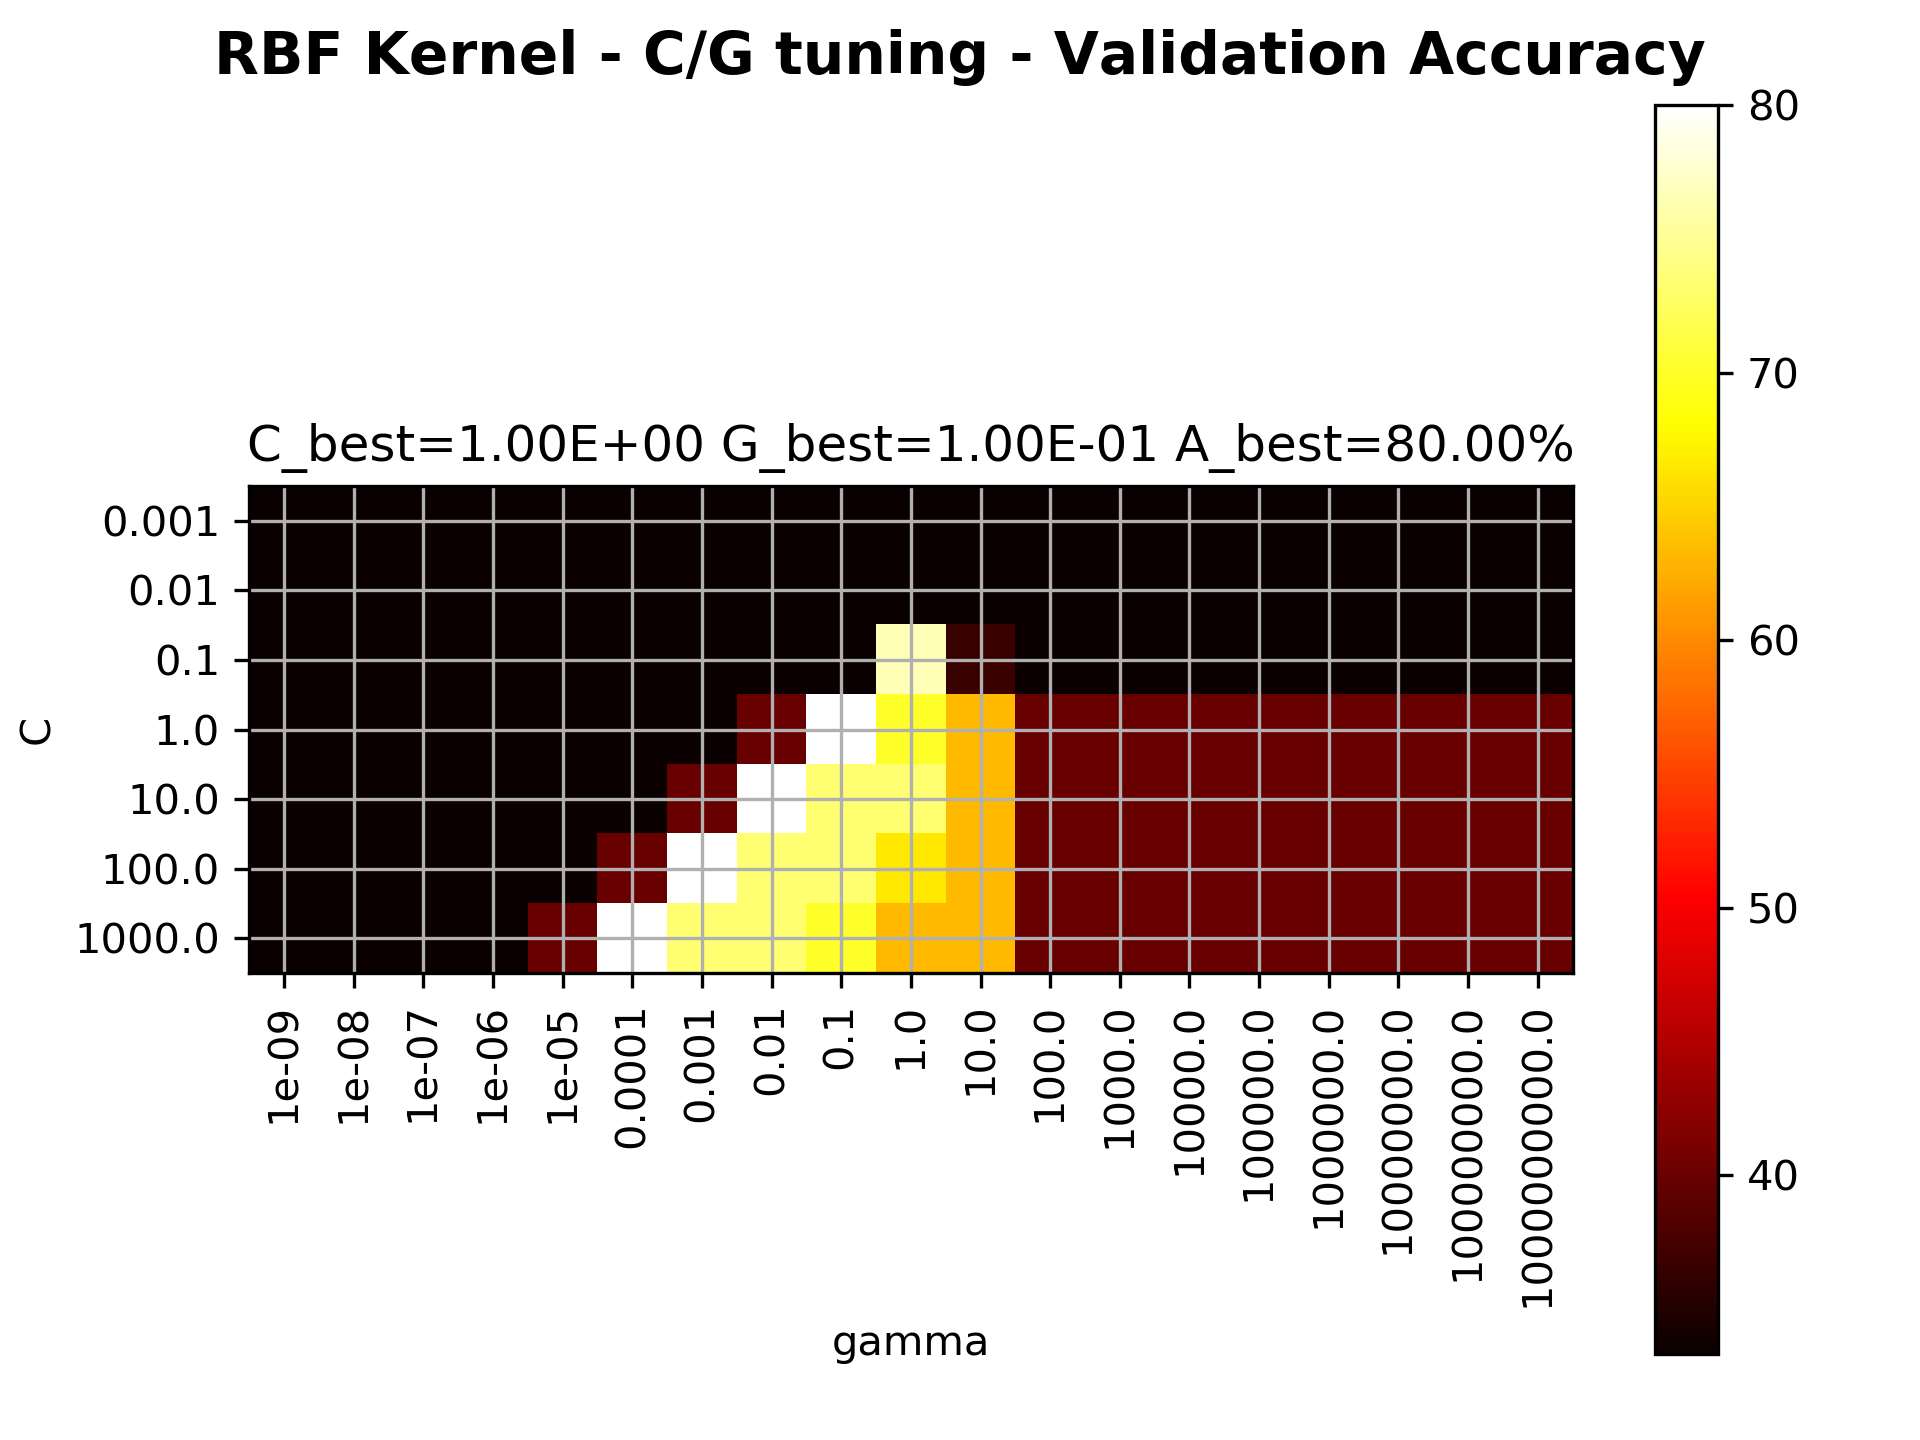
\includegraphics[width=0.7\paperwidth]{img/fig02d.png}
		\caption{Grid Search of C and Gamma in RBF Kernel SVM on Training set}
		\label{fig:rbf4}
	\end{figure}
	
	\begin{figure}[ht!]
		\centering
		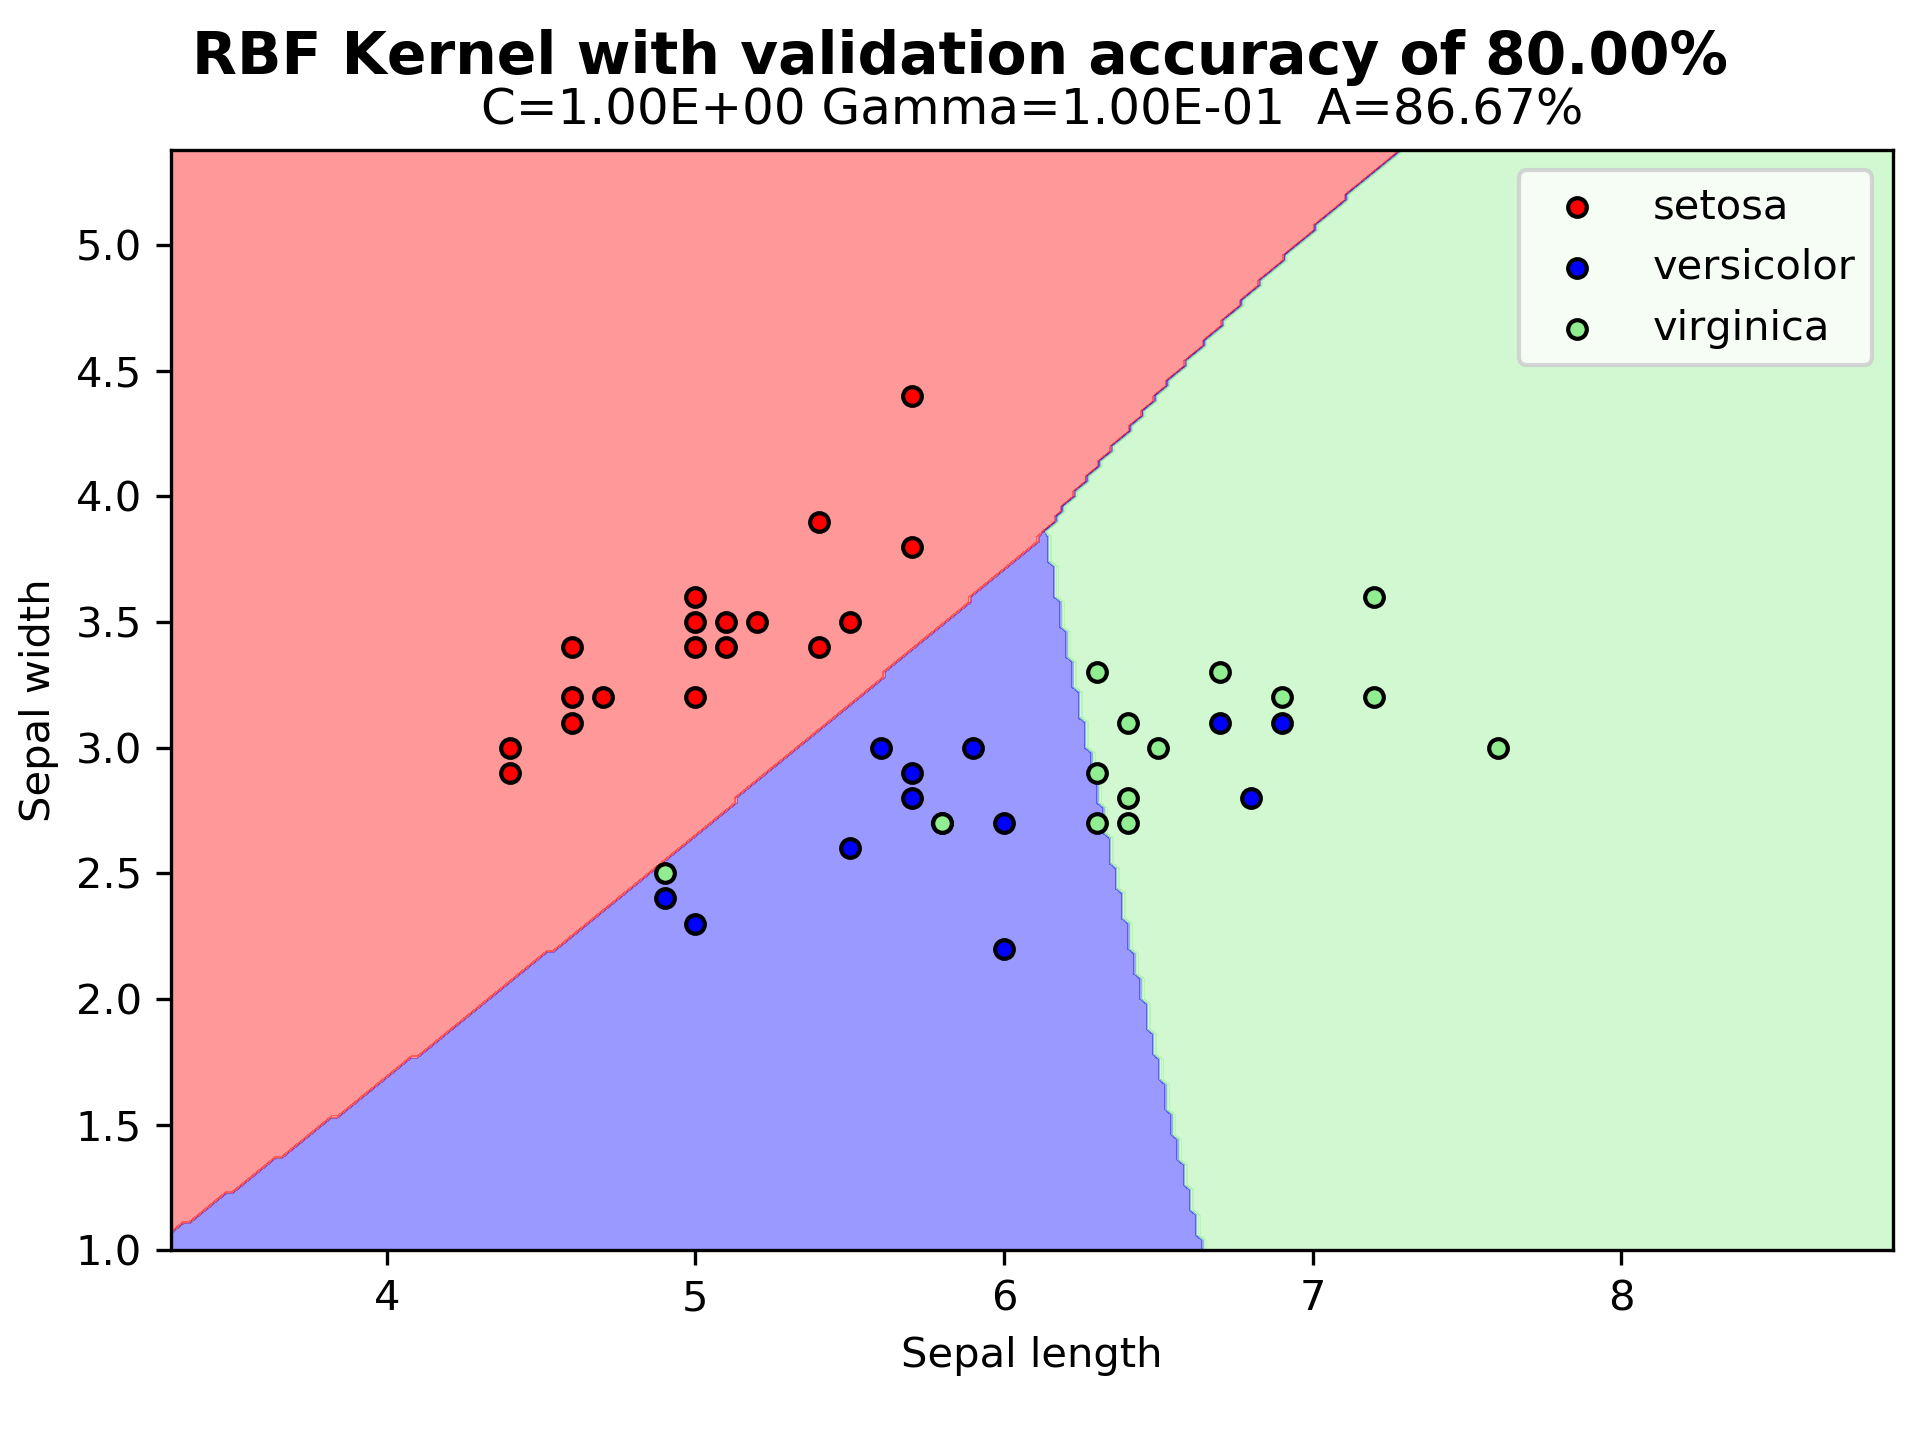
\includegraphics[width=0.7\paperwidth]{img/fig02e.png}
		\caption{Results on the test set}
		\label{fig:rbf5}
	\end{figure}
		
	\FloatBarrier
	
	\section{K-Fold}
		
	In the last part of the homework, I merged training and validation sets and I perfomed a \textbf{k-fold crossvalidation} with $k=5$ using \vref{lst:knn}.
	
	\lstinputlisting[ linerange={264-282},firstnumber=264s,label={lst:knn},caption={Validation using k-fold with $k=5$}]{../source_code/main.py}
	
	I obtained an in validation equal to $\boldsymbol{76.19\%}$, but a test accuracy $\boldsymbol{82.22\%}$ with a $\boldsymbol{C=1\mathrm{e}{2}}$ and $\boldsymbol{\gamma=1\mathrm{e}{-3}}$ as we can see in \vref{fig:knn}.
	
	The final score is good, although it is lower than some of the final scores found in previous sections. I tried to run the code multiple times changing \texttt{random\_state} and I have always found values from $75\%$ to $85\%$  (see \vref{final}).
	
	\begin{figure}[ht!]
		\centering
		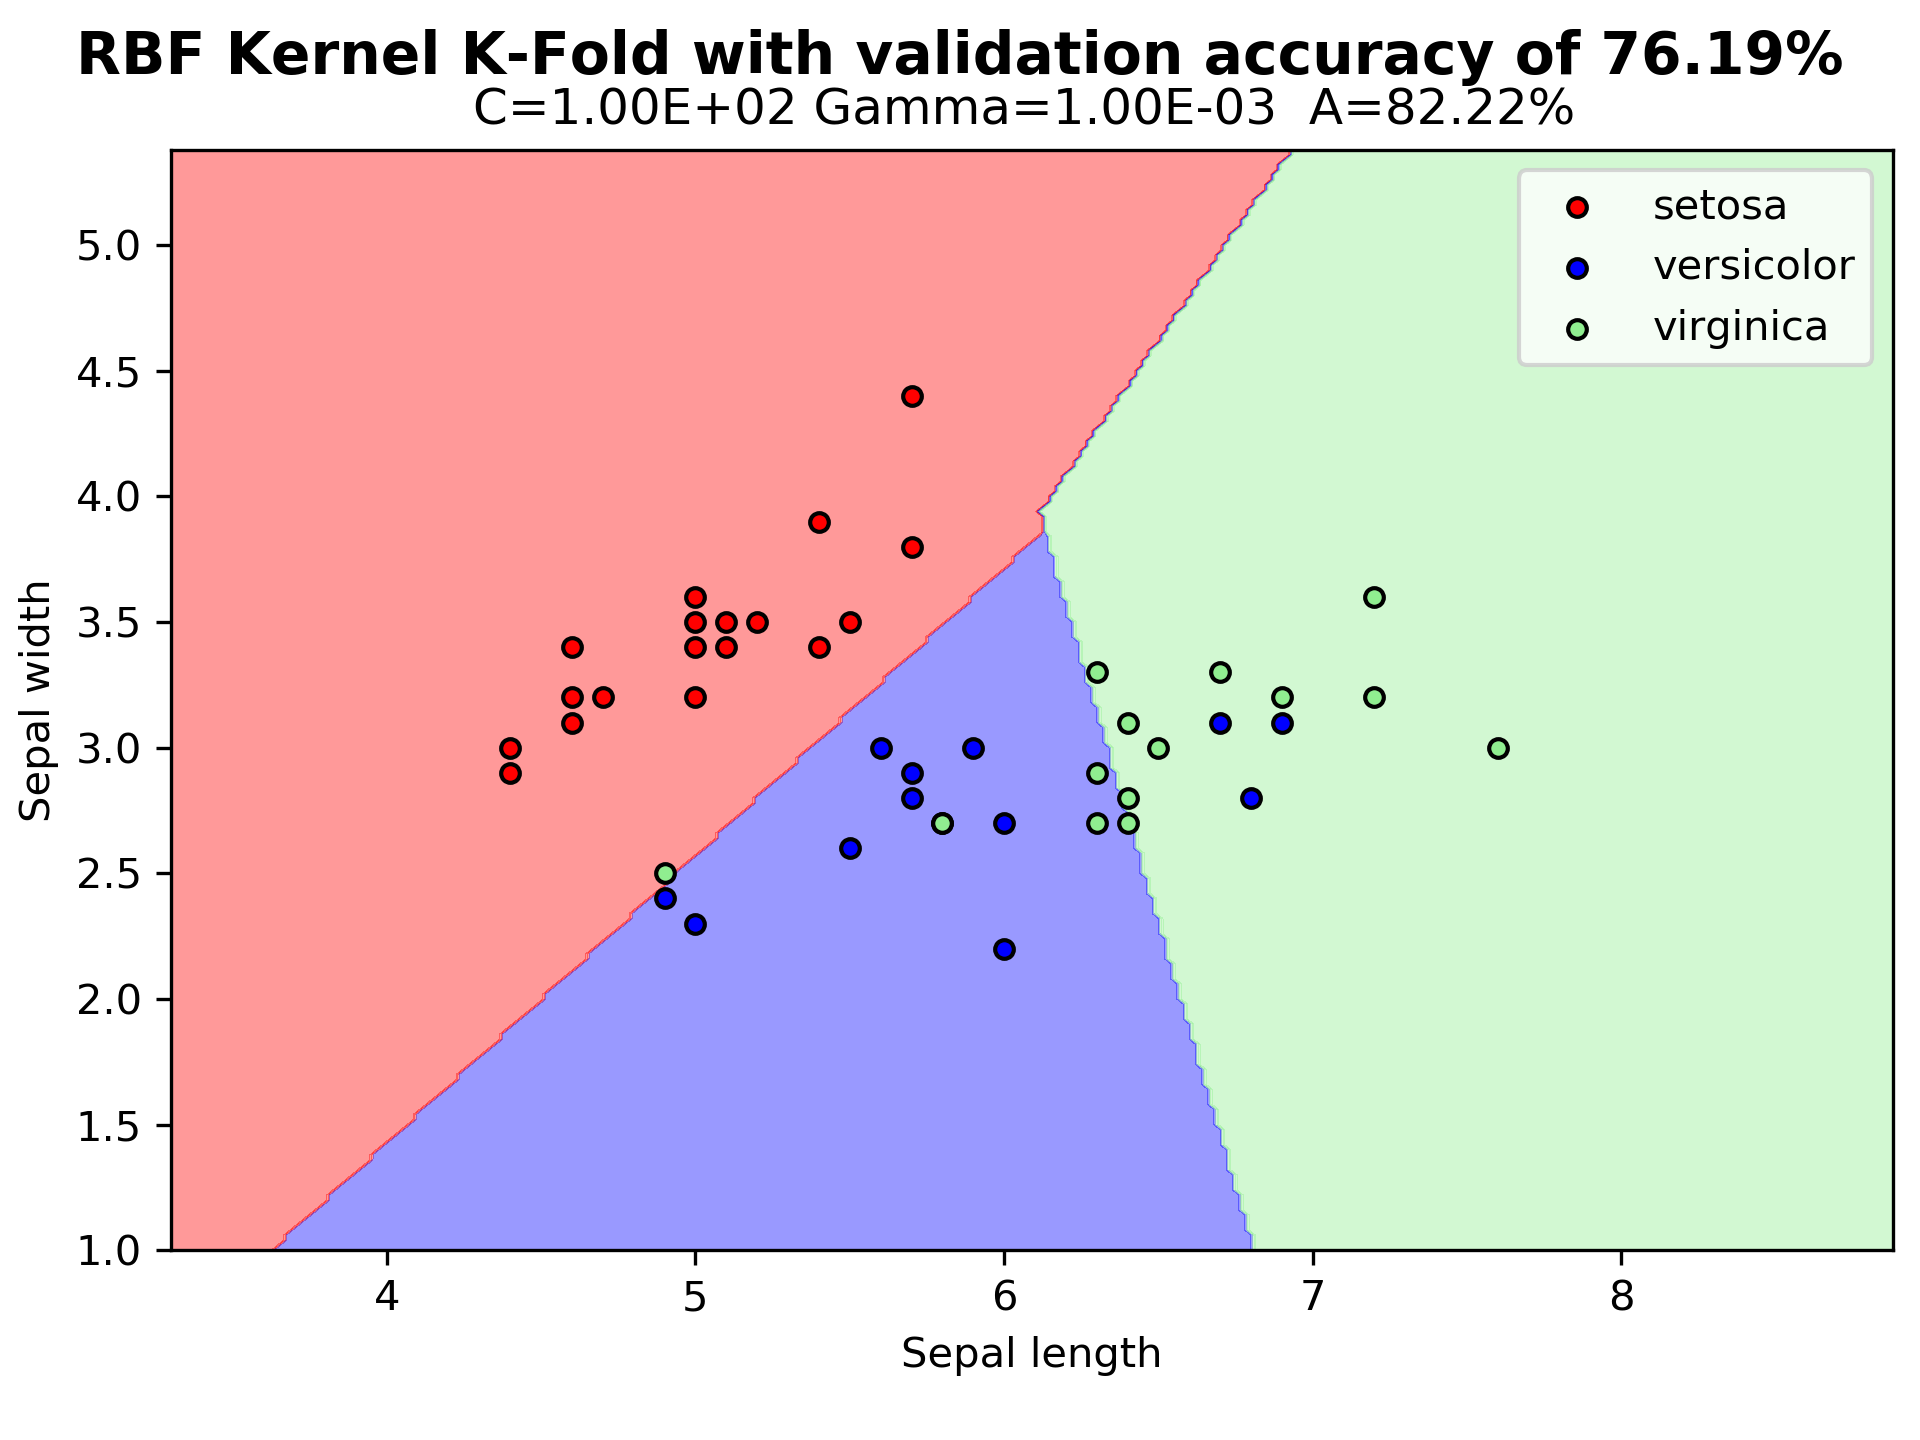
\includegraphics[width=0.5\paperwidth]{img/fig03.png}
		\caption{Results on the test set}
		\label{fig:knn}
	\end{figure}
	\section{Final Comments} \label{final}
	
	Because of the continuous variation of results for different \texttt{random\_state}, I decided to implement a simple Python script (\texttt{testing.py}) to calculate the average of the results of the three main type of parameter tuning in order to find something remarkable.
	The result obtained over 200 repetitions can be found in \vref{table1,table2}.
	\begin{table}[!h]
		\centering
		\caption{Accuracy distribution}
		\label{table1}
		\begin{tabular}{@{}lllll@{}}
			
			\toprule
			\textbf{Accuracy (\%)} (200 rep.)		& AVG Validation	& STD Validation	& AVG Test		& STD Test \\ \midrule
			Linear SVM				& $\approx80$	 	&  $\approx7$		& $\approx73$ & $\approx7$ \\
			RBF Kernel SVM			& $\approx82$	 	&  $\approx6$		& $\approx76$ & $\approx6$ \\
			RBF Kernel SVM (k-fold)	& $\approx81$	 	&  $\approx2$		& $\approx78$ & $\approx5$ \\ \bottomrule
		\end{tabular}
	\end{table}

	\begin{table}[!h]
		\centering
		\caption{Min and Max}
		\label{table2}
		\begin{tabular}{@{}lllll@{}}
			
			\toprule
			\textbf{Accuracy (\%)} (200 rep.)		& MIN Validation	& MAX Validation	& MIN Test		& MAX Test \\ \midrule
			Linear SVM				& $\approx60$	 	&  $\approx95$		& $\approx50$ & $\approx95$ \\
			RBF Kernel SVM			& $\approx60$	 	&  $\approx95$		& $\approx60$ & $\approx95$ \\
			RBF Kernel SVM (k-fold)	& $\approx75$	 	&  $\approx87$		& $\approx60$ & $\approx95$ \\ \bottomrule
		\end{tabular}
	\end{table}

	Now we have something that could be noteworthy: the first two type of parameter tuning algorithms have a larger variance than the last one. Therefore, the validation averages are almost the same, but the test ones no. Indeed, we can find an higher test accuracy on the third type.
	
	From these results, we can conclude that the validation done with k-fold crossvalidation is more stable than the other ones and it is useful to avoid overfitting problem.
		
	\section{Code Execution}
	\subsection{Requirements}
	\begin{itemize}
		\item Python 3
		\item All dependencies in \texttt{requirements.txt}.
		
		\texttt{\$ pip install -r requirements.txt} to install them
	\end{itemize}
	\subsection{Usage}
	\begin{itemize}
		\item \texttt{\$ python main.py}
		
		Execute the code
		
	\end{itemize}
	\subsection{Reproducibility}
	In order to reproduce the same data for this experiment you have to change the global variable \texttt{r\_state} (line) from \texttt{None} to $252894$ which is my badge number.

	\section*{Attachments}
	%Make sure to change these
	\begin{itemize}
		\item Source Code:
		\begin{itemize}
			\item \texttt{main.py}
			\item \texttt{requirements.txt}
			\item \texttt{testing.py}
		\end{itemize}
	\end{itemize}
	%\fi %comment me out
	
	
	
%	\begin{thebibliography}{9}
%		\bibitem{Robotics} Fred G. Martin \emph{Robotics Explorations: A Hands-On Introduction to Engineering}. New Jersey: Prentice Hall.
%		\bibitem{Flueck}  Flueck, Alexander J. 2005. \emph{ECE 100}[online]. Chicago: Illinois Institute of Technology, Electrical and Computer Engineering Department, 2005 [cited 30
%		August 2005]. Available from World Wide Web: (http://www.ece.iit.edu/~flueck/ece100).
%	\end{thebibliography}
	
\end{document}
